%%%%%%%%%%%%%%%%%%%%%%%%%%%%%%%%%%%%%%%%%%
% 宏包及宏定义
\documentclass{mcmthesis}
\mcmsetup{CTeX = false,   % 使用 CTeX 套装时,设置为 true
        tcn = 2218530, problem = C,
        sheet = true, titleinsheet = true, keywordsinsheet = true,
        titlepage = false, abstract = true}
\usepackage{newtxtext}  %\usepackage{palatino}
\usepackage{amssymb}
\usepackage{lipsum}
\usepackage{float}
\usepackage{graphicx}
\usepackage{subfigure}
\usepackage{array}
\usepackage{verbatim}
\newcommand{\upcite}[1]{\textsuperscript{\textsuperscript{\cite{#1}}}} 

%%%%%%%%%%%%%%%%%%%%%%%%%%%%%%%%%%%%%%%%%
% 标题
\title{Coping with the market: Trading Strategy Based on LSTM Time Series Prediction and Linear Programming}

%%%%%%%%%%%%%%%%%%%%%%%%%%%%%%%%%%%%%%%%%
% 开始正文
\begin{document}
% 首页summary sheet
\begin{abstract}    

We have witnessed the rapid growth of quantitative investment and there are many state-of-the-art techniques to help traders make the best strategy. Market traders buy and sell volatile assets frequently, with a goal to maximize their total return. There is usually a commission for each purchase and sale, while there is usually no cost to hold an asset. Two such assets are gold and bitcoin. In this paper, we developed a method to predict the future prices of gold and bitcoin so that a optimum trading strategy could be derived to maximize the final asset. 


We've established 2 models: \emph{Price Prediction Model Based on LSTM-CNN} and \emph{Trading Model Inspired by Dynamic Programming}.

Model(1): For price prediction, considering that the streams of daily prices of gold and bitcoin are typical time series, we adopted a deep learning model featuring a joint "LSTM-CNN" architecture to achieve high forecast accuracy. In order to reduce the influence of noise, we preprocessed the training data by smoothing the price curves with a rectangular window to achieve a better result and help training loss converge faster at the same time. We also took a suitable dynamic training mechanism to obtain the up-to-date model to ensure a decent prediction accuracy. Meanwhile, the training cost was also controlled within a reasonable and endurable range. The prediction results are shown in section ~\ref{details about ppm}.


Model(2): As for the trading method, we were inspired by dynamic programming to develop an algorithm which determined the next trading day and maintained optimum overall asset on that day. To find trading days, we looked for maximum and minimum prices in predicted price curves, which was more insightful, more guaranteed and more time-saving than running models everyday. Then, we optimized future assets with linear programming, which gave the best trading strategy for the current day according to the optimal principle of dynamic programming. Our model reached a profit rate over 7000\%, which is 139.4\% annualized rate of return. Trading history and the final result of assets are shown in section~\ref{details about ta}.


In addition, sensitivity analysis showed the total asset decreased roughly linearly as the commission rate multiplies. For example, when the commission rate was set to twice of its original value, the total asset shrunk to about 97.48\% of its original value.So our approach is robust to noises and commission rate changes. The sensitivity analysis is shown in figure ~\ref{fig:sensitivity result}. However, our rather greedy and risky approach requires high prediction accuracy rapid training of neural networks, so there's still much improvement to make in the future.


\begin{keywords}
Quantitative Transaction; Asset Configuration; Time Series Forecast; LSTM ; CNN; Dynamic Programming; Linear Programming
\end{keywords}
\end{abstract}
\maketitle

% 生成目录
\tableofcontents
\newpage    % 换页
%%%%%%%%%%%%%%%%%%%%%%%%%%%%%%%%%%%%%%%%%
% 第一部分,“引入”
\section{Introduction}
\subsection{Background }
Should you invest in Bitcoins? Bill Gates said yes but only if you are Elon Musk. Goldman Sachs(GS) said in a report that this February bitcoin could be more than double within the next five years, while 74\% of the professional investors surveyed by Bank of America saw bitcoin as a bubble last year. No matter what, historical price trend convinces us that investing in bitcoin and gold is promising.


Quantitative transaction is very popular since its birth because investment conducted by computer is objective and rational, and risks are effectively controlled. In recent years, it combines all sorts of time series prediction ranging from auto regression to deep learning, proposing multifarious investment strategies to help us maximize our assets in real-world markets.

% 问题的重新描述
\subsection{Problem Restatement}


This problem considers a trader who will start with \$1000 on 9/11/2016. On each trading day $i$, the trader has a portfolio consisting of cash, gold, and bitcoin, noted as $[C_i, G_i, B_i]$  in U.S. dollars, troy ounces, and bitcoins, respectively. The initial state is [1000, 0, 0] on 9/11/2016. The commission rate for each transaction (purchase or sale) is $\alpha_{gold} = 1\%$  and  $\alpha_{bitcoin} = 2\%$ of the amount traded. The problem is to help the trader develop a method which uses only the past stream of daily prices to determine each day if the trader should buy, hold, or sell his assets in the portfolio.


Specifically,  we need to:
\begin{itemize}
    \item Develop a that gives the \textbf{best} daily trading strategy during a five-year trading period till 9/10/2021.
    \item Try to prove our model provides the best strategy
    \item Analyse how sensitive our strategy is to transaction costs
    \item Communicate our strategy, model, and results to the trader
\end{itemize}


To simply the problem, we reasonably assume that the trader cannot lend cash or any other assets on each day, which means that the trader's cash on every should to be non-negative, and if the he/she attempts to make a sell, the amount of gold or bitcoin he/she sells should be no more than the amount he/she currently possesses.

% 考察D*_i的时候,如果要交易,那么交易按照今天的单价进行
% 10^-9的精度
% 约束条件现金数非负,也就是不能借钱,现金大于等于0,卖出的数量必须是已有的。整数

\subsection{Modeling framework}
Our solution to the problem can be divided into two parts:
\begin{enumerate}
    \item Price prediction with a deep learning model featuring a joint LSTM-CNN architecture
    \item Trading strategies algorithm inspired by dynamic programming
\end{enumerate}

\begin{figure}[htb]
    \centering
    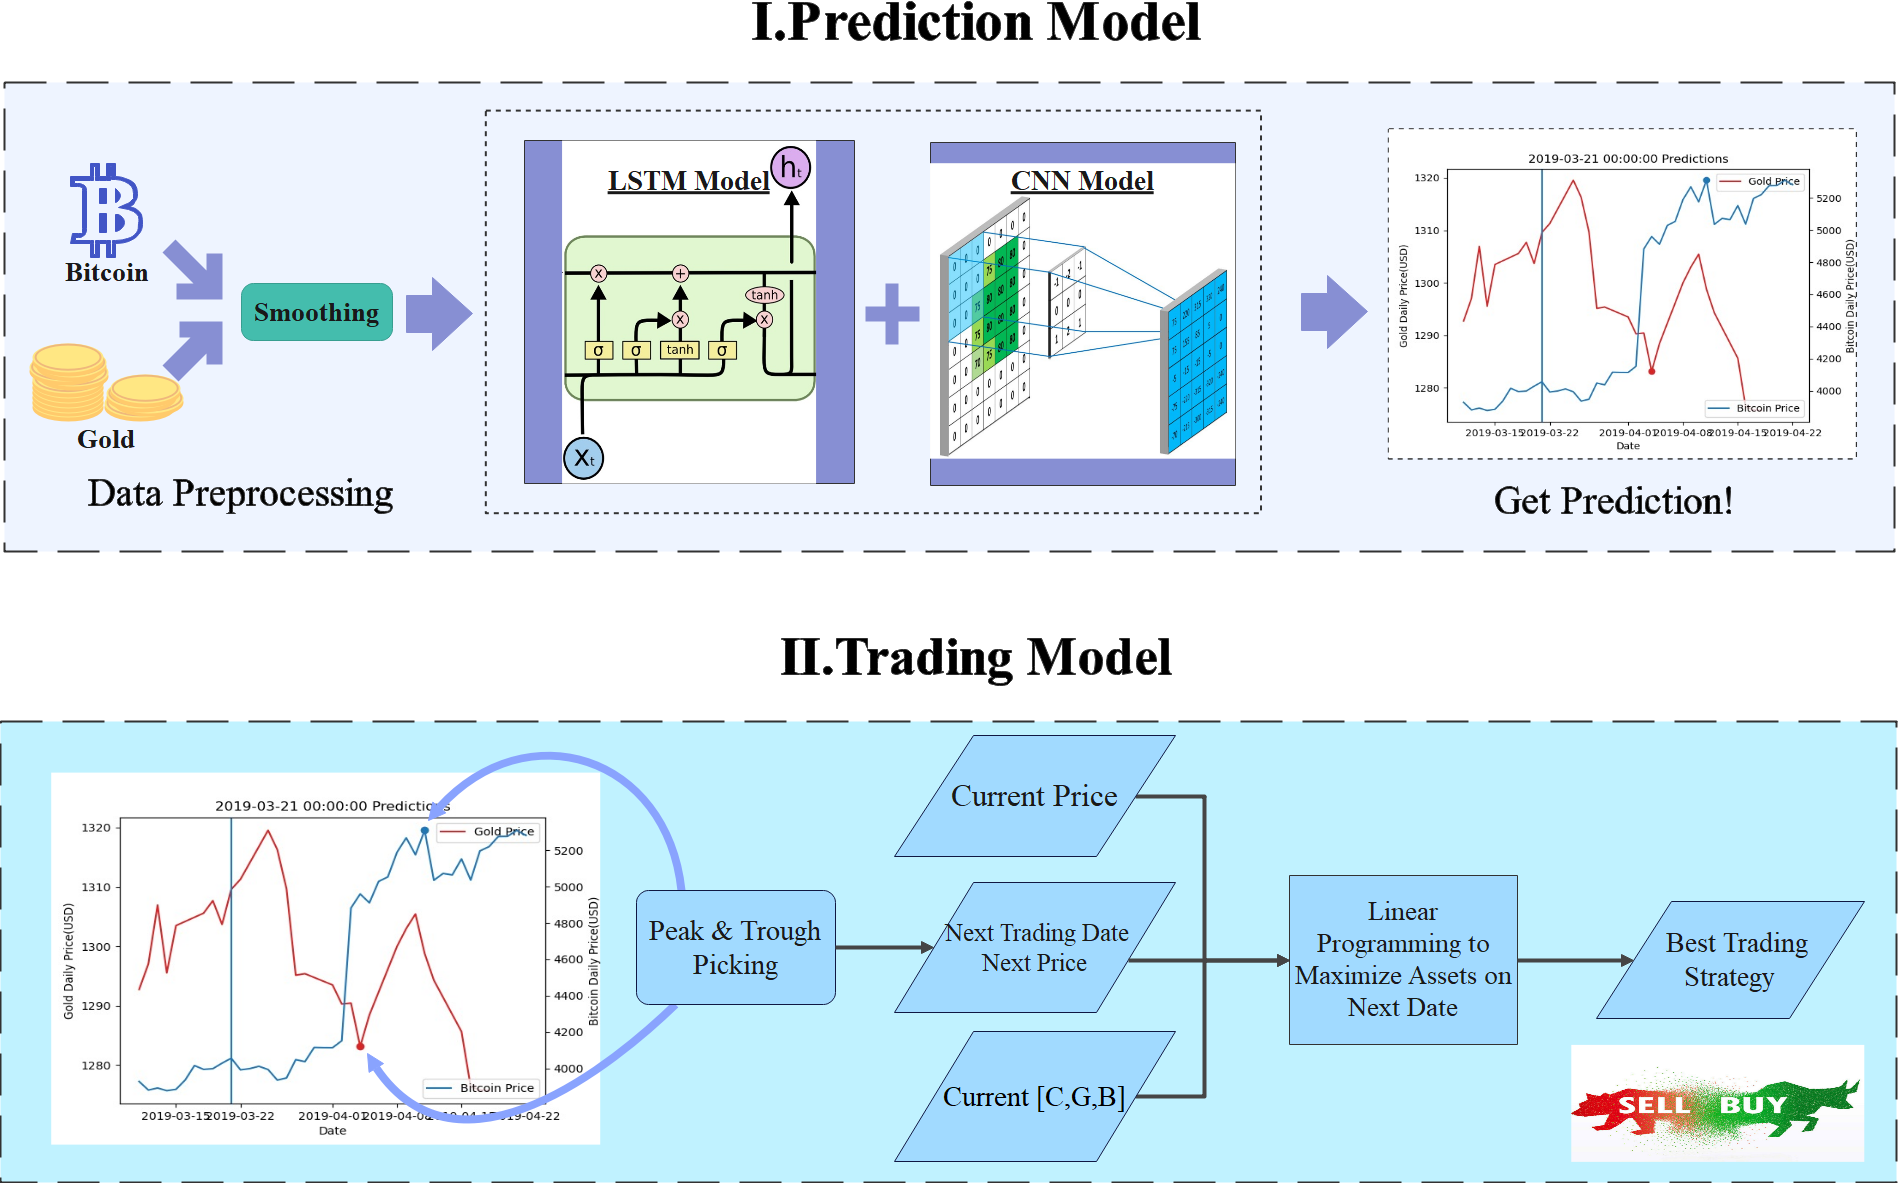
\includegraphics[width = 0.95\textwidth]{fig/model framework.png}  % 占文本可用宽度的0.8
    \caption{Modeling framework}
    \label{fig:framework}
\end{figure}

Our workflow is illustrated in figure~\ref{fig:framework}. Before we start trading, we wait for a particular length of time to observe gold and bitcoin prices since we need sufficient data to train the prediction model. When enough training data is collected, we train the deep learning prediction model with a joint \emph{LSTM-CCN} architecture and use the model to predict gold and bitcoin prices in the future. Before we put training data into the model, we smooth the price curve since there is noise on it, especially for bitcoin. After we attain future price curves, we pick their peaks and troughs future days as potential future trading dates. Then we use linear programming maximize total assets on each candidate trading day and find out the day with the biggest asset along with the corresponding trading strategy for today. We complete today's trading based on the derived strategy and jump to the previously picked corresponding trading day. We repeat this procedure till the end of the trading period.



% 更新模型?

%%%%%%%%%%%%%%%%%%%%%%%%%%%%%%%%%%%%%%%%%
% 第二部分,假设和记号定义
\section{Assumptions \& Notations}
\subsection{Assumptions}
As mentioned in the problem restatement above, the assumptions can be formalized as:
\begin{enumerate}
    \item The amount of cash on each day in the 5-year trading period is non-negative, i.e.
    \begin{equation}
        C_{d_i} \geq 0 \quad \forall d_i \in \bold{D}
    \end{equation}
    \item The amount of gold and bitcoin sold each trading day is no more than the amount of gold and bitcoin in the current asset, i.e.
    \begin{equation}
        O^G_{d_i^*} \geq -G_{d_i^*} \quad \forall d_i^* \in \bold{D^*}
    \end{equation}
    \begin{equation}
        O^B_{d_i^*} \geq -B_{d_i^*} \quad \forall d_i^* \in \bold{D^*}
    \end{equation}
    \item The gold and bitcoin prices are considered known before the trading decision is made on every day during the trading period, i.e. $P^G_i$ and $P^B_i$ can be treated as given conditions on day i, ${\forall d_i \in \bold{D}}$.
\end{enumerate}

\subsection{Notations}
The main notations we defined during our modeling are shown in 
Table ~\ref{tab:notations}:
\begin{table}[htbp]
\caption{Notations}
\label{tab:notations}
\centering
	\begin{tabular}{c|c}
		\hline
		 \txtbf{Symbol}       \txtbf{& Description}   
		\\ \hline
		$d_i$            &The $i$th day                               \\
		$d_i^*$        &The $i$th trading day
		\\
		$\bold{D}$   &The set of all days in the trading periods \\
		$\bold{D^*}$   &The set of all trading days
		\\
		$A_{i}$        &Total assets on day i                               \\
		$C_{i}$        &Amount of cash on day i                             \\
		$G_{i}$    &Amount of gold on day i                             \\
		$B_{i}$        &Amount of bitcoin on day i                          \\ 
		$P_{i}^G$      &Gold price on day i                                 \\
		$P_{i}^B$      &Bitcoin price on day i                              \\
		$O_i^G$        &Amount of gold purchased(+) or sold(-) on day i     \\  
		$O_i^B$        &Amount of bitcoin purchased(+) or sold(-) on day i  \\
		$\alpha_{gold}$    &Commission rate of gold transaction                 \\
		$\alpha_{bitcoin}$    &Commission rate of bitcoin transaction              \\
		\hline
	\end{tabular}
\end{table}

%%%%%%%%%%%%%%%%%%%%%%%%%%%%%%%%%%%%%%%%%
% 第三部分,预测模型介绍
\section{Price Prediction Model}
\emph{Prediction} is the most essential part in the problem pipeline. Our price prediction model features a \textbf{joint LSTM + CNN architecture} which is expected to perform well on time series forecasts according to previous research. Here, we propose a method to predict future prices of gold and bitcoin using previous observations as training data. Our prediction model involves three parts: \emph{data preprocessing}, \emph{LSTM+CNN model} and \emph{dynamic training mechanism}.

\subsection{ Data preprocessing}\label{data preprocessing}

\begin{figure}[htb]
    \centering
    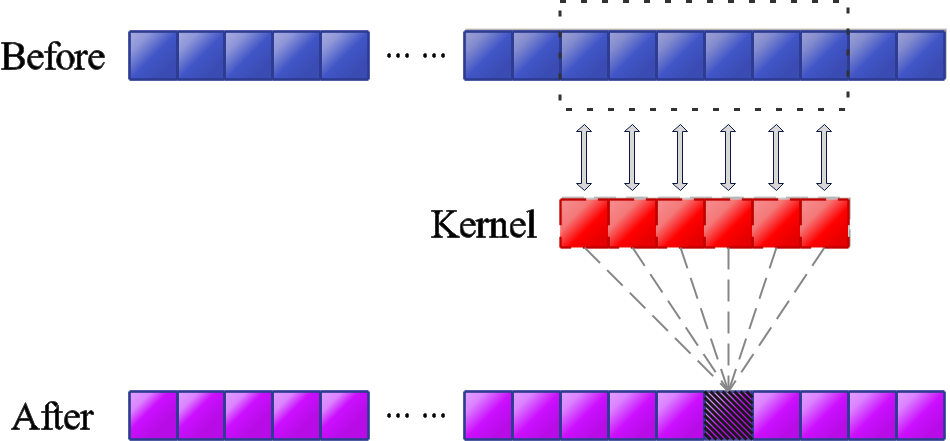
\includegraphics[width = 0.6\textwidth]{fig/smooth process.png}  
    \caption{smooth process}
    \label{fig:smooth process}
\end{figure}

If we look at the price curves, it's not difficult to spot noise. Moreover, the convergence speed of training loss when using raw price data (as shown in figure ~\ref{before smooth}) is slower than that if the data is smoothed with a rectangular window before it's put into the neural network (as shown in figure ~\ref{after smooth}). Therefore, we use a convolution window to preprocess price data (shown in figure ~\ref{fig:smooth process}) and the epoch number used in model training can be reduced.

% 插入2子图的模板,用subfigure{}函数
\begin{figure}[htb]
\centering
\subfigure[Before smooth]{
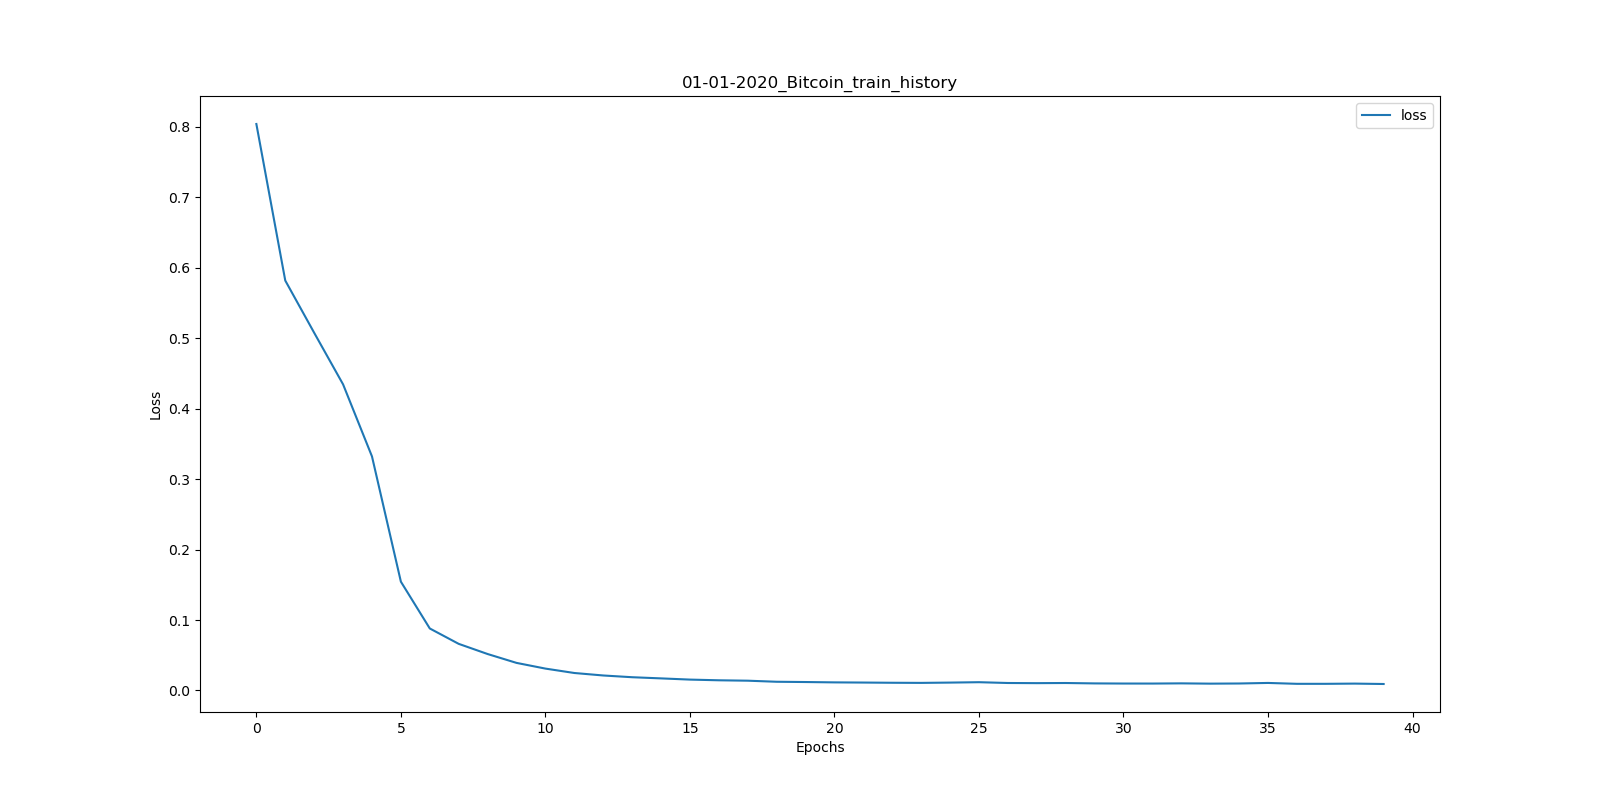
\includegraphics[width = 6in]{fig/convergence speed of training loss before smooth.png}
\label{before smooth}
}
\subfigure[After smooth]{
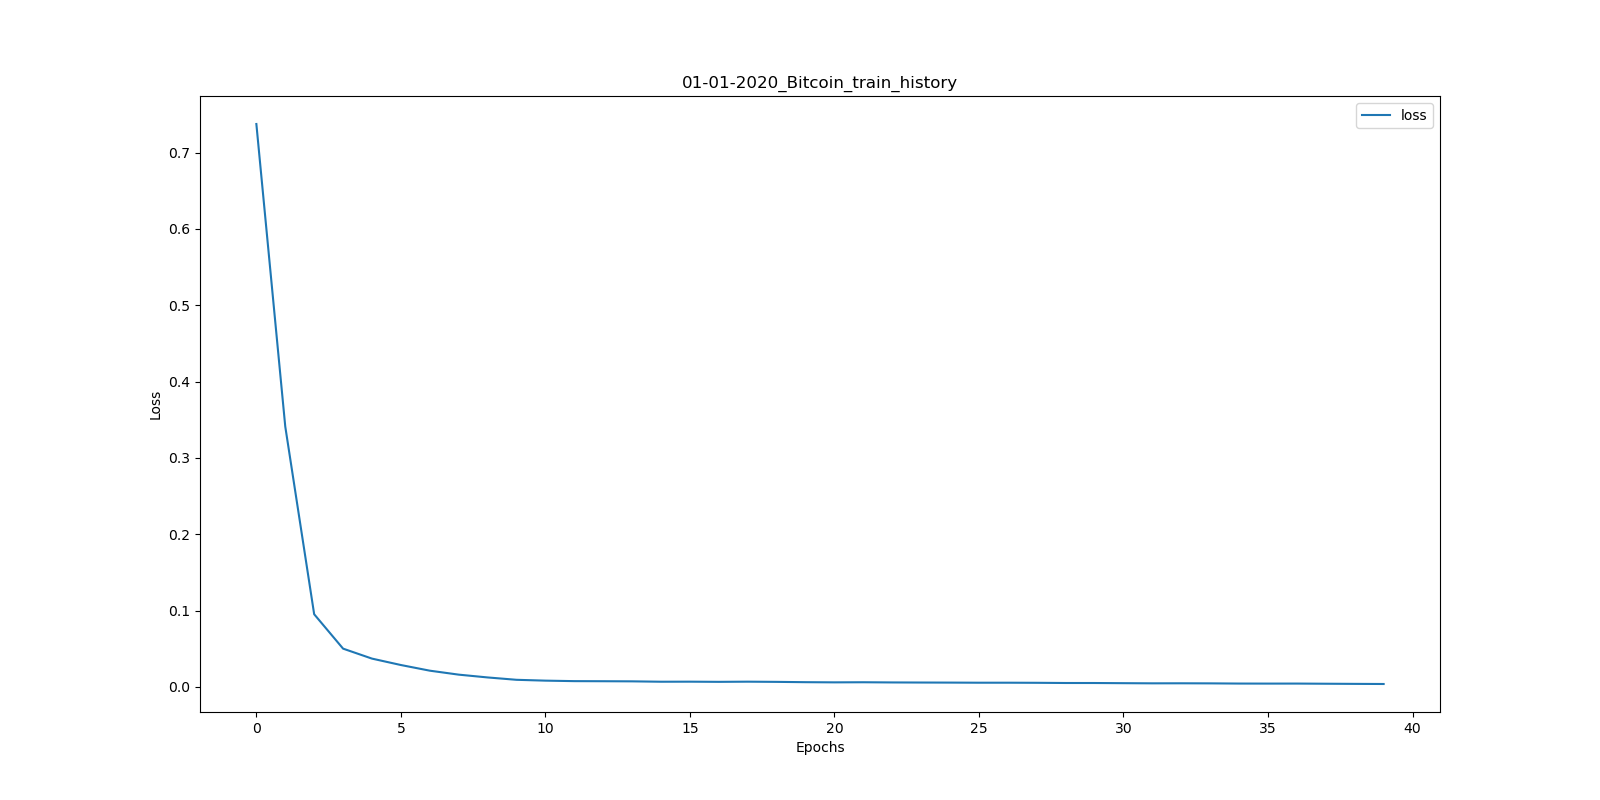
\includegraphics[width = 6in]{fig/convergence speed of training loss after smooth.png}
\label{after smooth}
}
\caption{Contrast regarding smooth method}
\label{fig:smooth}
\end{figure}


\subsection{ LSTM+CNN model}
 Previous research have proposed several tips to our approach. In 1997, Sepp Hochreiter \emph{et al}. \cite{1} invented the LSTM model to solve the problem of vanishing gradient and  exploding gradient during long time series prediction. In 2019, Zhanhong He \emph{et al}.\cite{2}, and in 2020, Ioannis E. Livieris \emph{et al}.\cite{3} illustrated that the utilization of LSTM layers along with additional convolutional layers could provide a significant boost in increasing the gold price forecasting performance. Besides, in 2021, GuoSihan \cite{4} pointed out that the stream of bitcoin price is non-linear and in traditional economics, this currency is considered to be completely supplying inelastic, which means there is no apparent \emph{linear} relationship between the production of bitcoin mining and its price. Take all the information into consideration, we've decided to build a "LSTM + CNN" model to predict gold and bitcoin prices, the structure of which is shown in figure~\ref{fig:network structure}.

\begin{figure}[htb]
    \centering
    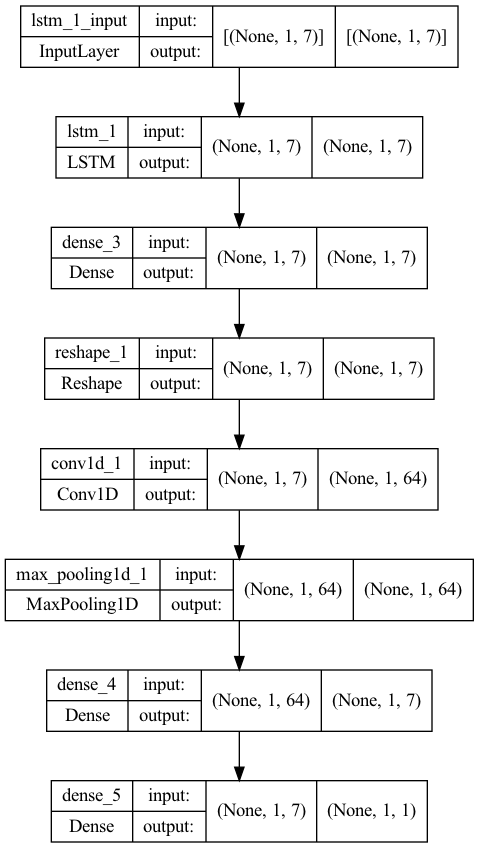
\includegraphics[width = 0.5\textwidth]{fig/network structure.png} 
    \caption{Network structure}
    \label{fig:network structure}
\end{figure}


\subsection{Dynamic training mechanism}
In the paper \cite{4}, author Guo Sihan used some kind of  dynamic method in model training to keep it up to date, and each time step is predicted by the model trained by price data right before that step. This method is also adopted in our approach.


Due to the lack of training data at the beginning, we have to wait $d_{wait}$ days (eg,120) to accumulate price data to train our prediction model for the first time. Later, all the data before $d_i^*$ will be taken to train the model, which will be based on the \emph{previous} one rather than training it starting from scratch. Meanwhile, the training epic will be reduced. Thus, not only the continuity of the model can be guaranteed, but also it will save lots of time. The $d_i^*$ mentioned above refers to the $i$th trading day we choose, the first one is the $121$th day, and the subsequent $d_i^*$ will be selected according to the conclusion given by the trading model in section ~\ref{derive next trading day}.

\subsection{Prediction results}\label{details about ppm}
As we can see from figure ~\ref{fig:prediction result}, the prediction result matches well with the actual data, except for about a few days delay. Although the usage of smooth on raw data doesn't bring about much improvement in terms of prediction result, we have already shown the benefit of smoothing in the reduction of training time in subsection  ~\ref{data preprocessing}.

\begin{figure}[htb]
\centering
\subfigure[without smooth]{
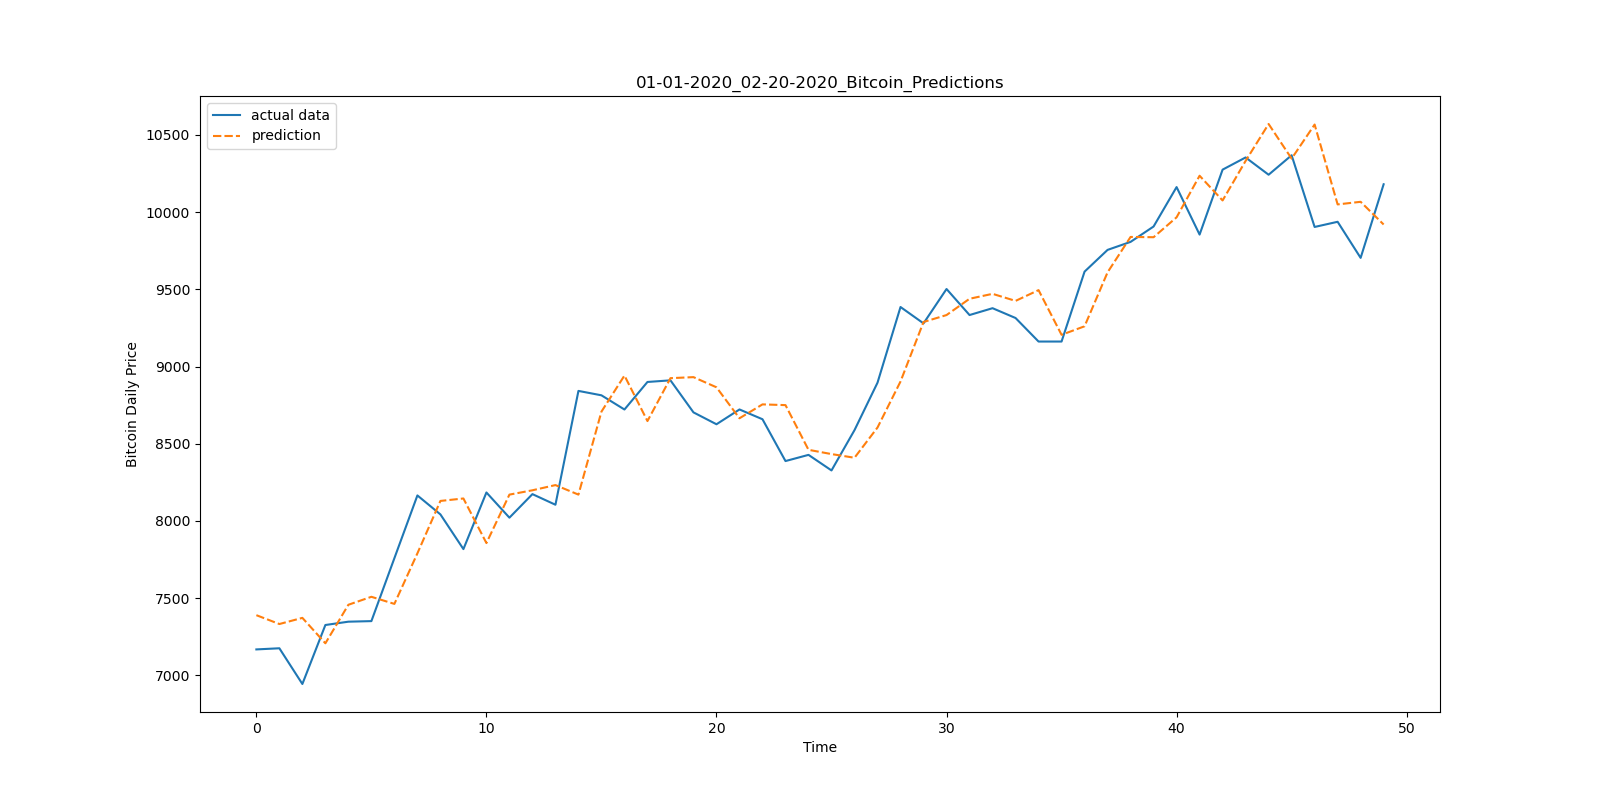
\includegraphics[width = 5.5in]{fig/prediction result without smooth.png}
\label{without smooth}
}
\subfigure[with smooth]{
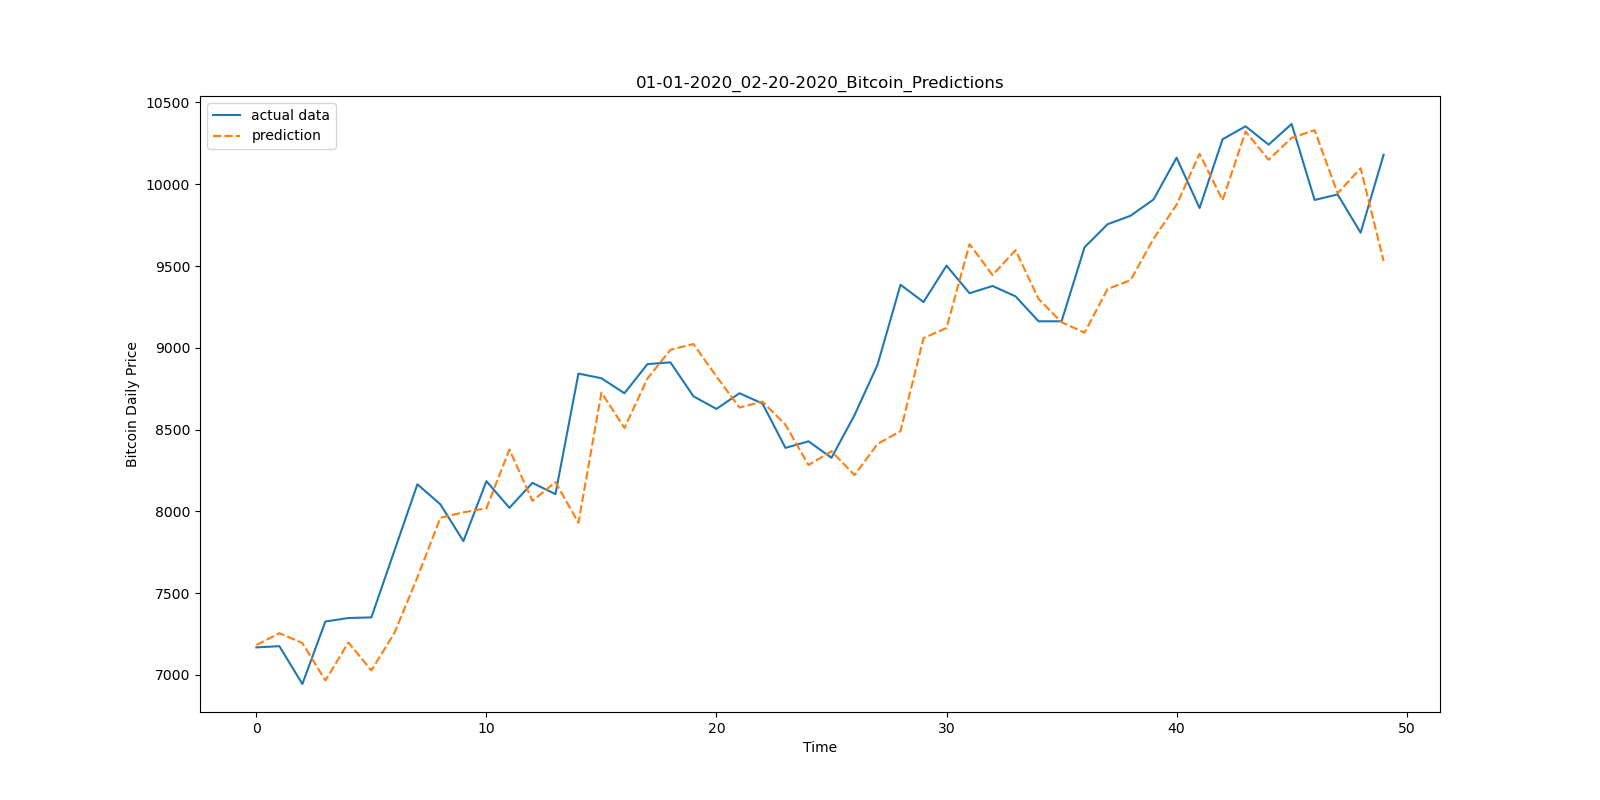
\includegraphics[width = 5.5in]{fig/prediction result with smooth.png}
\label{with smooth}
}
\caption{Prediction result regarding smooth method}
\label{fig:prediction result}
\end{figure}

%%%%%%%%%%%%%%%%%%%%%%%%%%%%%%%%%%%%%%%%%
% 第四部分,决策模型介绍
\section{Trading Algorithm}
Every day in the trading period, our goal is to maximize the trader's final asset. In other words, we make the decision of whether to trade or not on a particular day to maximize the asset in the future, regardless of the profit or loss of the current trade with respect to previous trades. Our core idea is that the past cannot be changed (note that we've assumed that the price is given before trading on each day, the current price information on each day is in the "past" as well, since it won't change), therefore we have to make the trading decision that will maximize the overall assets on a particular point of time in the future. Inspired by \emph{dynamic programming}, we present an algorithm to derive the best trading strategy for everyday. 

\subsection{Overview of the Trading Algorithm}
The pipeline of our algorithm is illustrated in figure~\ref{fig:trading algorithm pipeline}. We start by waiting for several days to accumulate training data, then we join the loop by training the prediction model and making future price predictions. We analysis the predicted price curve and determine the next trading date and the predicted price on that day. We optimize the asset on the next trading day with the aid of linear programming(since the target function of asset is linear) to get the optimum trading strategy for today. Now, we can purchase and sell asset according to the strategy derived and jump to the next trading date which was determined when analyzing the predicted price curve and start a new cycle of the loop. When we reach the end of the 5-year trading period, we jump out of the loop and finish the whole trading. The core parts of the algorithm are interpreted in the following sections in detail.

\begin{figure}[htb]
    \centering
    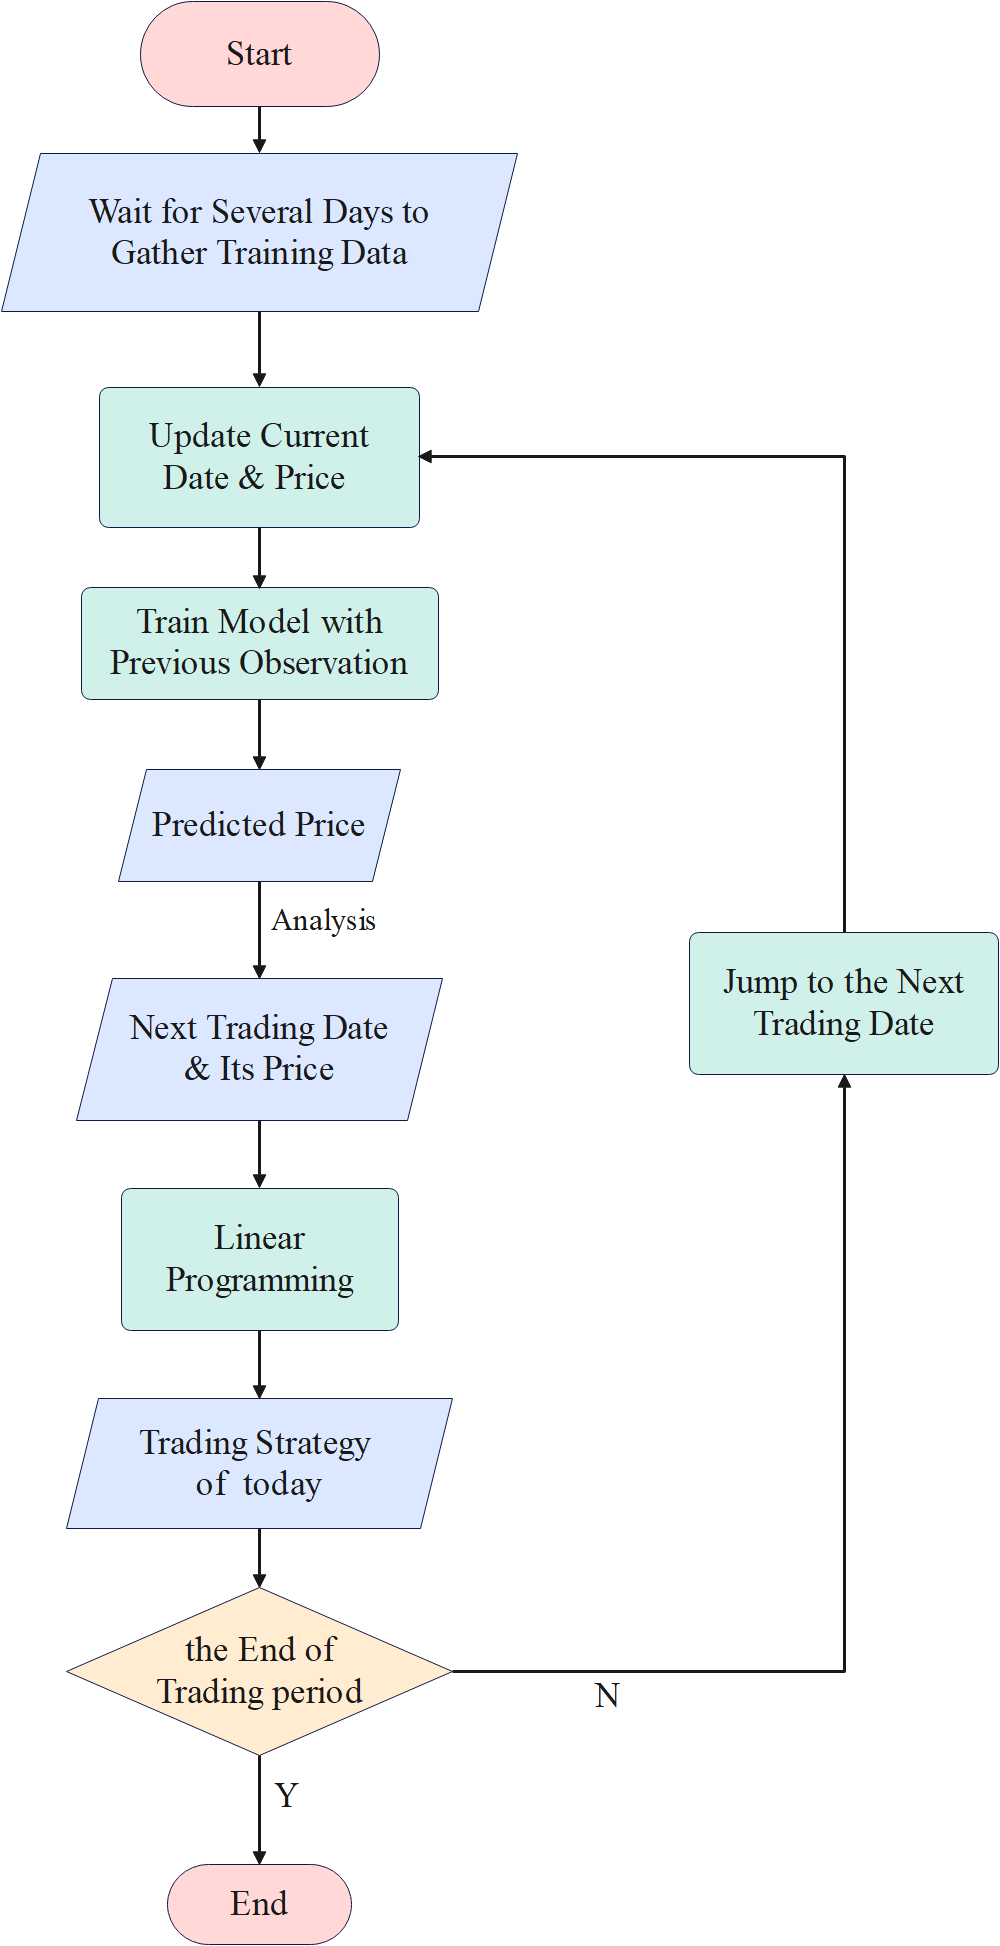
\includegraphics[width = 0.5\textwidth]{fig/trading algorithm pipeline.png}
    \caption{Trading algorithm pipeline}
    \label{fig:trading algorithm pipeline}
\end{figure}


\subsection{Analysis of prediction price}
Before we demonstrate our analysis method, let us discuss the basic idea of trading. We can only gain profit when we purchase asset at a lower price and sell them at a higher price. The price difference is what we are relying on. Suppose the amount of a particular asset we possess is $O$, the lower price and higher price is $P_low$ and $P_high$ respectively and the commission rate is $\alpha$,. The condition for gaining profit is
\begin{equation}
    P_{high}O - (P_{low}O + P_{high}O)*\alpha > P_{low}O
\end{equation}
thus
\begin{equation}
    P_{high} > \frac{1+\alpha}{1-\alpha}·P_{low}
\end{equation}
The profit is ${O*(P_{high}(1-\alpha) - P_{low}(1+\alpha))}$.


In short, we are looking for larger price differences in the predicted data to get larger profit. Therefore, we look for peaks and troughs in the predicted price curve and address the corresponding date as potential next trading date, as shown in figure ~\ref{fig:example of peak and trough locating}. The green dots showed the price on 2017-09-15, the left side of the green dots are previous observations, while the right side are predictions. The peak and trough are picked by locating the maximum and minimum price in the predicted curve within a given range of time. Our next step is to choose a specific date as next trading date and determine the trading strategy of today.


\begin{figure}[htb]
\centering
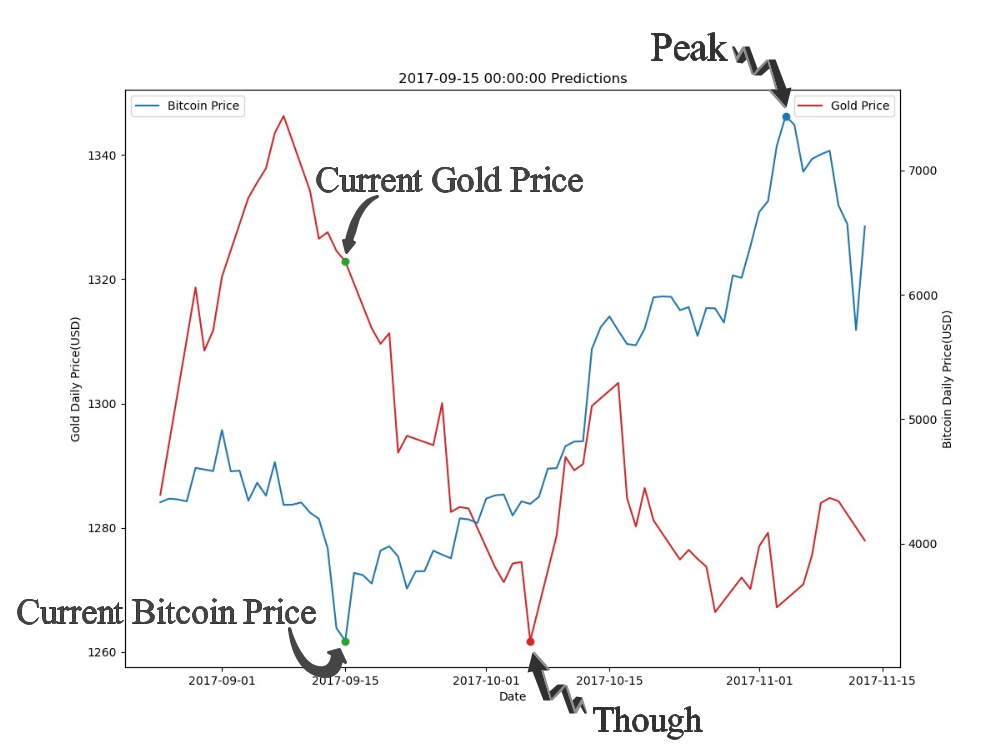
\includegraphics[width =  0.85\textwidth]{fig/example of peak and trough locating.png}
\caption{Example of peak and trough locating}
\label{fig:example of peak and trough locating}
\end{figure}

\subsection{Derive trading strategy}\label{derive next trading day}
This section shows how we determine the next trading day among the candidates and trading strategy for the current day. Inspired by \bold{dynamic programming}, we treat every trading day as a state and try to optimize the asset on the next state, i.e. the next trading day. 


Suppose one of the potential next trading dates we found out is $d^*_{i+1}$ with predicted gold price $P^G_{d^*_{i+1}}$ and bitcoin price $B^G_{d^*_{i+1}}$. The current assets is $[C_{d^*_{i}}, G_{d^*_{i}}, B_{d^*_{i}}]$ and the current day price is $P^G_{d^*_{i}}$ and $B^G_{d^*_{i}}$. Suppose we trade $O^G_{d^*_i}$ troy ounces of gold and $O^B_{d^*_i}$ bitcoins. The asset on $d^*_{i+1}$ is
\begin{equation}
\begin{aligned}
A_{d^*_{i+1}} &= C_{d^*_{i}} - O^G_{d^*_i} · P^G_{d^*_{i}} - O^B_{d^*_i}·P^B_{d^*_{i}} - \alpha_{gold}·O^G_{d^*_i}·P^G_{d^*_{i}}  - \alpha_{bitcoin}·O^B_{d^*_i}·P^B_{d^*_{i}} \\ 
& \quad + (G_{d^*_{i}} + O^G_{d^*_i})·P^G_{d^*_{i+1}} + (B_{d^*_{i}} + O^B_{d^*_i})·P^B_{d^*_{i+1}}
\end{aligned}
\end{equation}


To optimize the about function to get maximum asset on $d^*_{i+1}$, we can simply use \bold{linear programming} since the function is linear and the boundaries are determined by our assumptions:
\begin{equation}
        C_{d^*_{i}} - O^G_{d^*_i} · P^G_{d^*_{i}} - O^B_{d^*_i}·P^B_{d^*_{i}} - \alpha_{gold}·|O^G_{d^*_i}|·P^G_{d^*_{i}} - \alpha_{bitcoin}·|O^B_{d^*_i}|·P^B_{d^*_{i}} \geq 0 
\end{equation}
\begin{equation}
    O^G_{d^*_i} \geq -G_{d^*_{i}}
\end{equation}
\begin{equation}
    O^B_{d^*_i} \geq -B_{d^*_{i}}
\end{equation}


Notice that there is an absolute value function in one of the boundaries, so we need to treat the linear programming problem with classified discussion. However, it is not a hard task for programming with Python. We treat every potential next trading date with the about method and choose the day that has the optimum asset as the next trading date and trade with the corresponding trading strategy. After that we can jump to next trading date and start a new loop.


%%%%%%%%%%%%%%%%%%%%%%%%%%%%%%%%%%%%%%%%%
% 第五部分,结果
\section{Results}\label{details about ta}
Using the given data and proposed model, we simulated the training process with Python (we trained the prediction model with TensorFlow). The trading history is shown in the figure~\ref{trading history}. The \$1000 asset eventually turned into \$78658.58 after five years' trading!

\begin{figure}[htb]
\centering
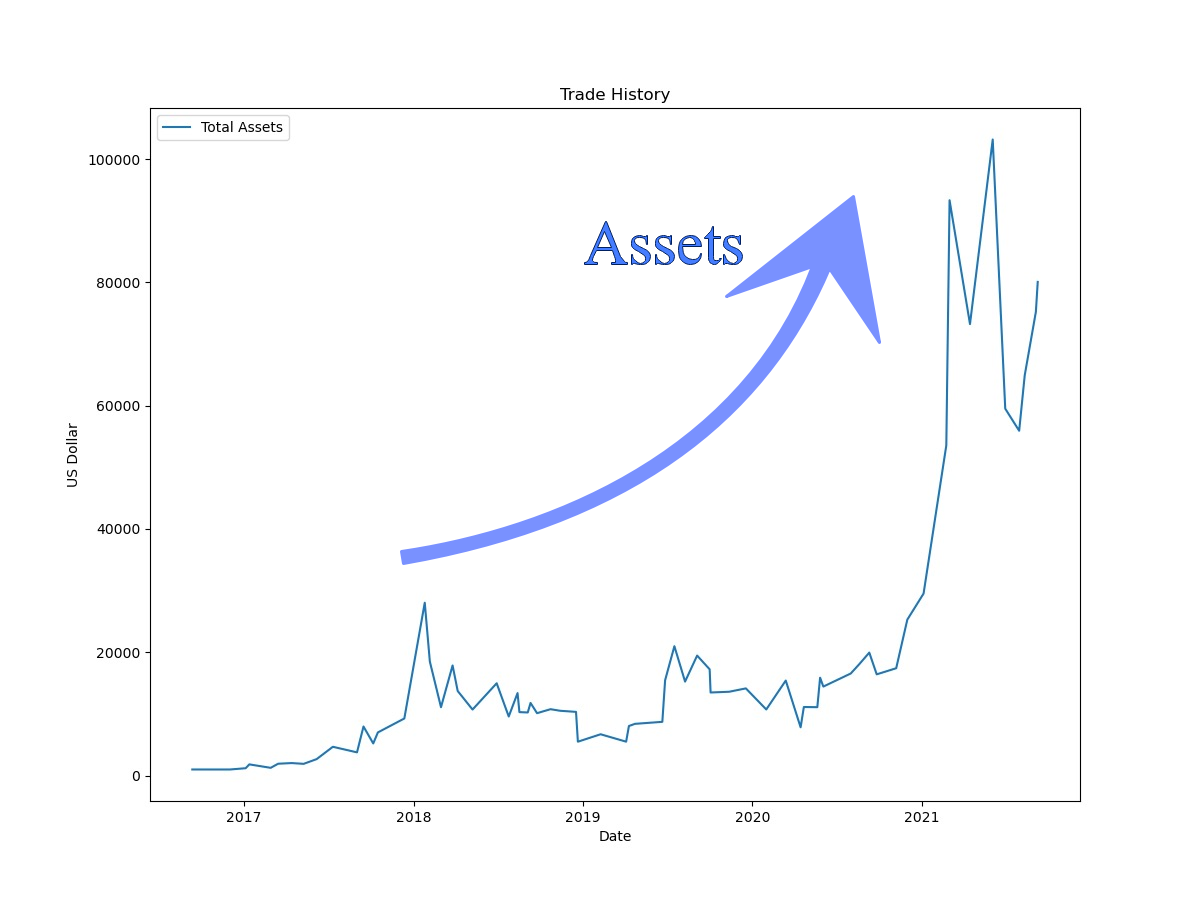
\includegraphics[width = 0.75\textwidth]{fig/trading history.png}
\caption{Trading history}
\label{trading history}
\end{figure}

%%%%%%%%%%%%%%%%%%%%%%%%%%%%%%%%%%%%%%%%%
% 第六部分,敏感度分析
\section{Sensitivity analysis}
In this section, we will discuss our model's sensitivity to commission rates. We change the commission rates and run simulations to get the following results. 


As shown in figure ~\ref{fig:sensitivity result}, our final asset increases slightly with the reduction of commission rates, which means that the relative change is tiny. So our model is robust and insensitive to commission rates.


\begin{figure}[htb]
\centering
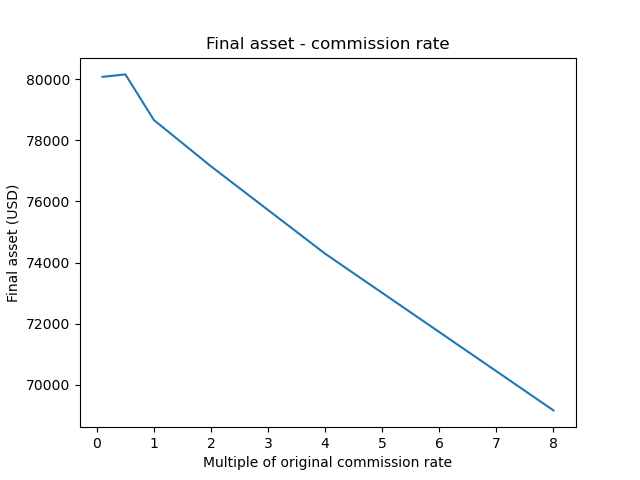
\includegraphics[width =  0.75\textwidth]{fig/sensitivity result.png}
\caption{Sensitivity to commission rate}
\label{fig:sensitivity result}
\end{figure}

%%%%%%%%%%%%%%%%%%%%%%%%%%%%%%%%%%%%%%%%%
% 第七部分,评估
\section{Model Evaluation}
\subsection{Strengths}
    \begin{enumerate}
    \item According to our simulation, our model performs well on the given price data and is robust to different commission rates. The overall profit rate is 7765.86\% with $\alpha_{gold} = 1\%$  and  $\alpha_{bitcoin} = 2\%$.  
    
    \item Our model deals with noise by smoothing the training data. This measure allows our model to be \textbf{robust against noise}.
    
    \item Our model features LSTM architecture in price prediction model. LSTM performs especially well on long time series forecast, which equip our model with a stronger prediction ability and greater accuracy.
\end{enumerate}

\subsection{Weaknesses}
    \begin{enumerate}
    \item Our trading strategy aims to maintain a maximum asset on each coming trading day. It's actually a very greedy and risky approach. Since it desires maximum profit, it puts all asset at stake in order to gain profit. There will be huge loss when the trading strategy is erroneous.
    
    \item Our method requires frequent training of neural networks in order to make accurate and up-to-date predictions. The training process consumes a lot of computing resources, and it takes a certain amount of time. Thus our method is not suitable for assets with rapid price fluctuations.
    
    % \item
    
\end{enumerate}
%%%%%%%%%%%%%%%%%%%%%%%%%%%%%%%%%%%%%%%%%
% 第八部分,备忘录
\newpage
\section{A memorandum to the trader}
\memoto{trader}
\memofrom{2218530}
\memosubject{Trading Strategy}
\memodate{\today}
%\logo{\LARGE Bullshit}
\begin{memo}[Memorandum]

Dear Sir/Madam,

Thanks for reading this memorandum. We are a research team working on quantitative investing. We are honored to introduce our marketing strategy to you. This model will help you obtain maximum benefit with your portfolio consisting of cash, gold, and bitcoin [C, G, B] in U.S. dollars, troy ounces, and bitcoins, respectively, in a market where gold and bitcoin can be traded. We will be more than glad if you can make lots of money based on our approach. 


Firstly, let us show you with the fantastic results of our simulation. To make it simple, we turn 1000 dollars into 78658.58 dollars when applying our approach on bitcoin and gold market from 09.2016 to 09.2021 (as shown in figure ~\ref{fig:to trader1})! It means that you can expect a 139.4\% annualized rate of return. In comparison to bank, the rate is 39.83 times of that for 5-year regular savings in the bank, which is just around 3.5\%.


\begin{figure}[htb]
\centering
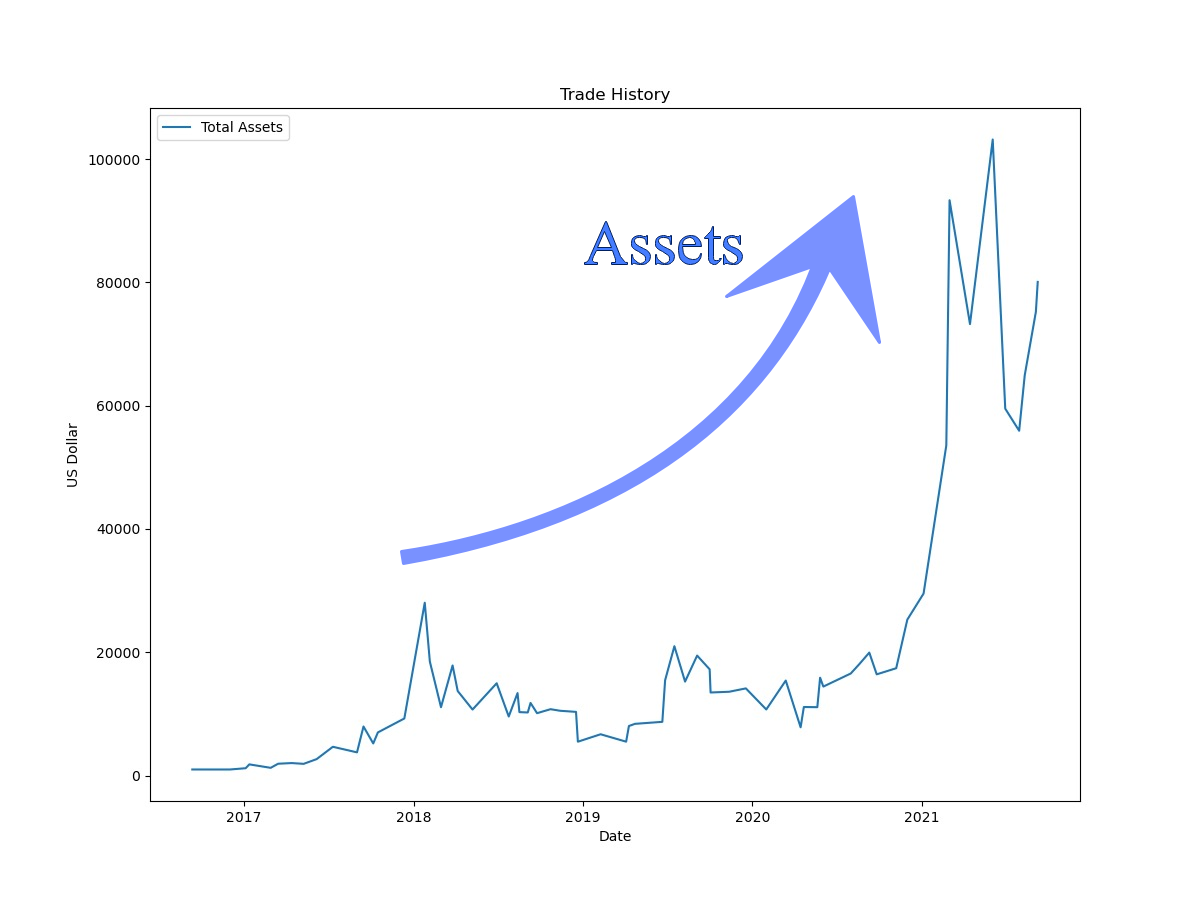
\includegraphics[width = 0.7\textwidth]{fig/trading history.png}
\caption{results}
\label{fig:to trader1}
\end{figure}

Secondly, we develop a method to predict the future prices of gold and bitcoin so that a optimum trading strategy can be derived to maximize the final assets. The frame of this approach is shown in figue ~\ref{fig:to trader2}

\begin{figure}[htb]
    \centering
    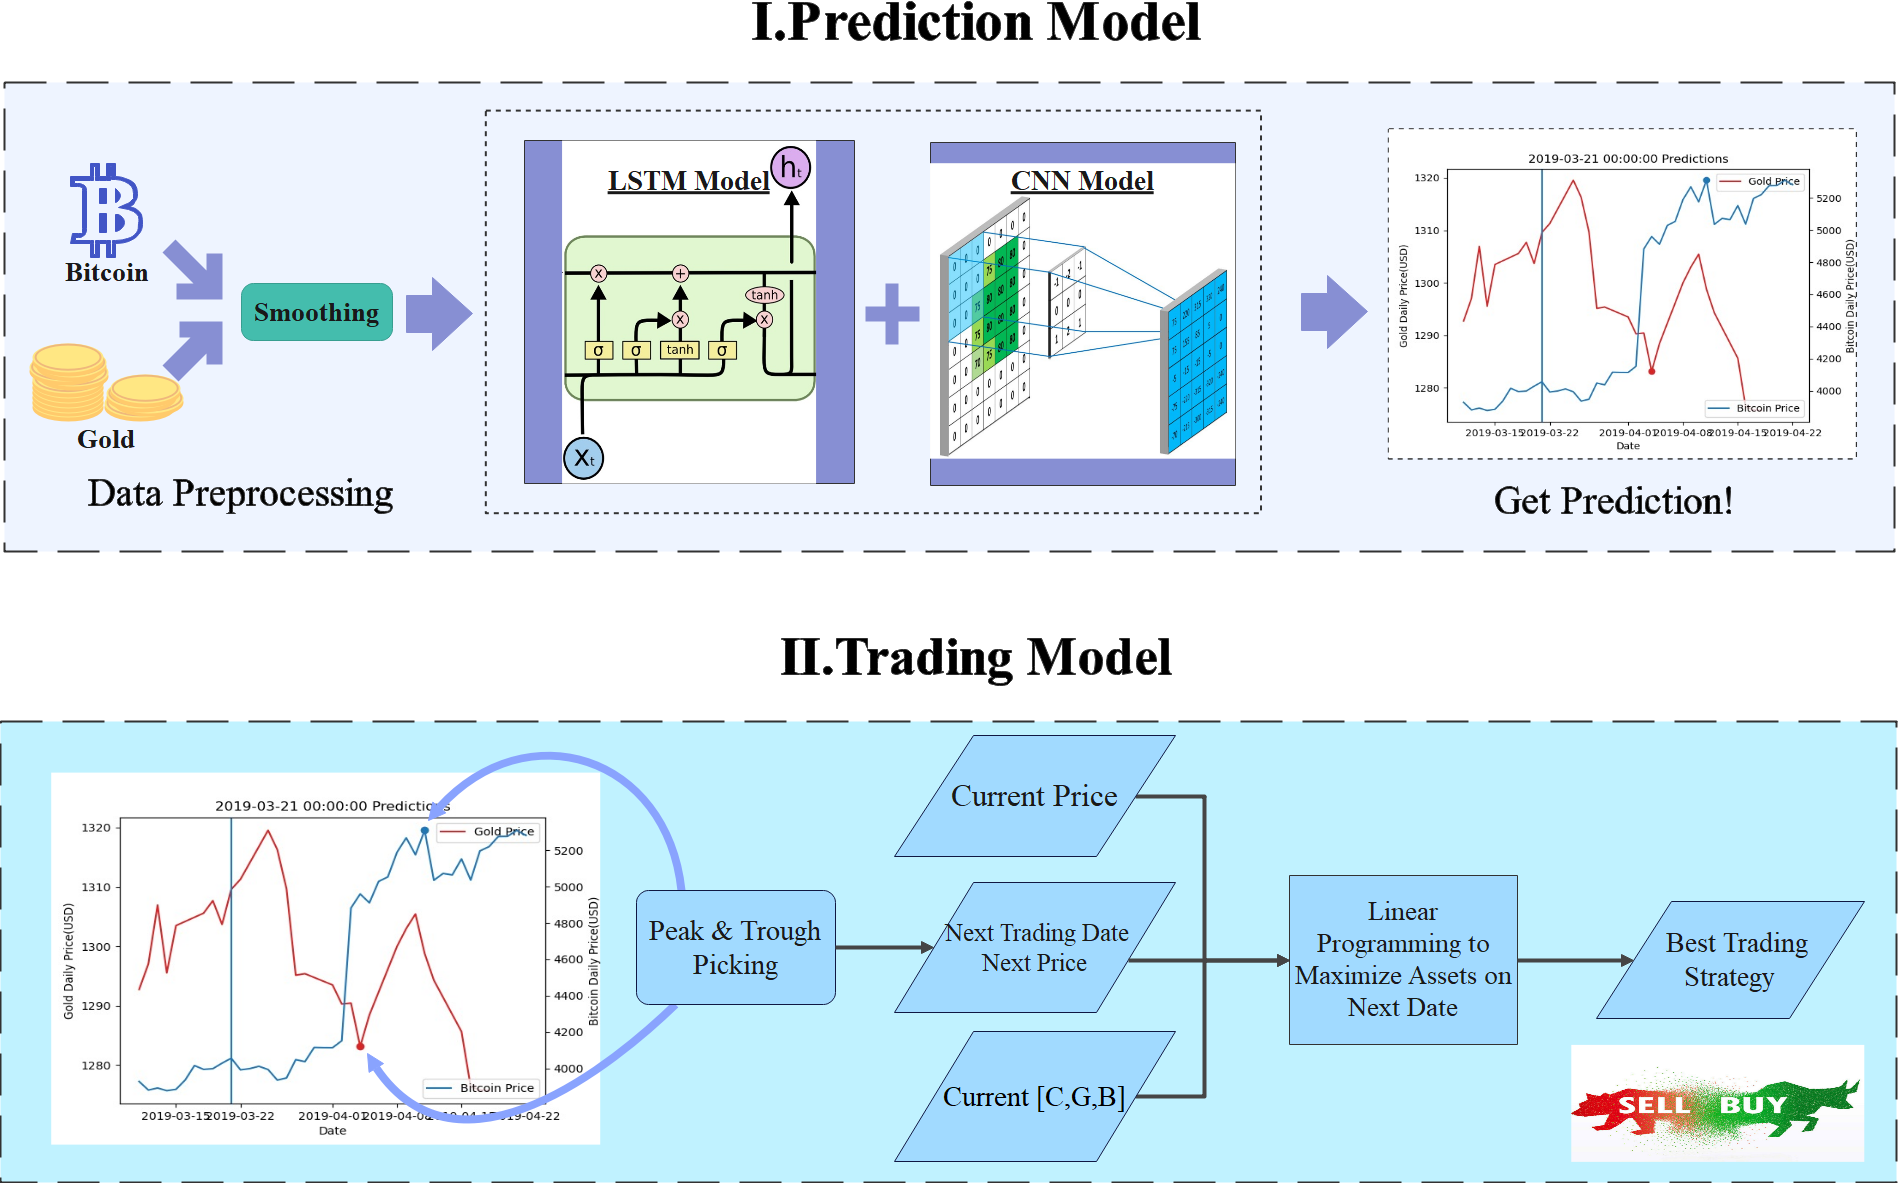
\includegraphics[width = 0.95\textwidth]{fig/model framework.png}  % 占文本可用宽度的0.8
    \caption{Modeling framework}
    \label{fig:to trader2}
\end{figure}

Our approach contains two models:


Model(1): For price prediction, we adopt a deep learning model featuring a joint "LSTM-CNN" architecture to achieve high forecast accuracy. We also preprocess the training data by smoothing the price curves with a rectangular window to achieve a better result and help training loss converge faster at the same time. Then we take a suitable dynamic training mechanism to obtain the up-to-date model to ensure a decent prediction accuracy. Meanwhile, the training cost is also controlled within a reasonable and endurable range. 



Model(2): As for the trading method, we are inspired by dynamic programming to develop an algorithm which determine the next trading day and maintain optimum overall asset on that day. To find trading days, we look for maximum and minimum prices in predicted price curves, which is more insightful, more guaranteed and more time-saving than running models everyday. Then, we optimize future assets with linear programming, which gives the best trading strategy for the current day according to the optimal principle of dynamic programming.


In addition, sensitivity analysis showed the total asset decreases roughly linearly as the commission rate multiplies. For example, when the commission rate is set to twice of its original value, the total asset shrinks to about 97.48\% of its original value. So our approach is robust to noises and commission rate changes. However, our rather greedy and risky approach requires high prediction accuracy rapid training of neural networks, so there's still much improvement to make in the future.


To wrap up, we provide you with this up-to-date quantitative investment approach. I wish you make good use of it and good luck!

\end{memo}



\begin{thebibliography}{99}%参考文献
\bibitem{1}Sepp Hochreiter, Jurgen Schmidhuber(1997). LONG SHORT-TERM MEMORY.
\bibitem{2}Zhanhong He, Junhao Zhou, Hong-Ning Dai, Hao Wangy, (2019).Gold Price Forecast based on LSTM-CNN Model.
\bibitem{3}Ioannis E. Livieris1, Emmanuel Pintelas1, Panagiotis Pintelas, (2020).A CNN–LSTM model for gold price time-series forecasting.
\bibitem{4}Guo Sihan, (2021).Research on Bitcoin price prediction and trading strategy based on improved recurrent neural network.
\end{thebibliography}

\end{document}